\documentclass[10pt,a4paper]{article}
\renewcommand{\baselinestretch}{1.0}
\usepackage{cite}
\usepackage[dvips]{graphicx}
\usepackage{psfrag}
\usepackage{color}
\usepackage[cmex10]{amsmath}
\usepackage{amsfonts}
\usepackage[font=footnotesize, captionskip=10pt]{subfig}
\usepackage{tikz}
\usepackage{flushend}
\usepackage{times}
\usepackage[margin=1.5cm]{geometry}
\usepackage[slovak]{babel}
\usepackage[utf8]{inputenc}
\usepackage[T1]{fontenc}

\usepackage{multirow}
\usepackage{colortbl}

\pagestyle{empty}

\hyphenation{net-works}
\newtheorem{remark}{Remark}

\begin{document}

\title{Playing multiple games using deep reinforcement learning}
\author{Michal Chovanec, Ondrej Šuch}
\date{}
\maketitle
\thispagestyle{empty}

{\bf Abstract}
In this paper we presents deep Q network (DQN) playing multiple games with the same weights - six ATARI games.
We trained network by randomly changing games after several interations, using deep reinforcement learning.
For comparison, we also trained common DQN. Instead of using 8x8 or 4x4 kernels as in (cite Atari DQN and Doom paper)
we used only 3x3 kernels, and much lower of feature maps in layers. This network is much more parameter efficient.
As results we present training score progress and network feature maps usability for each game.


\section{Introduction}


\begin{figure}[htb!]
\centering
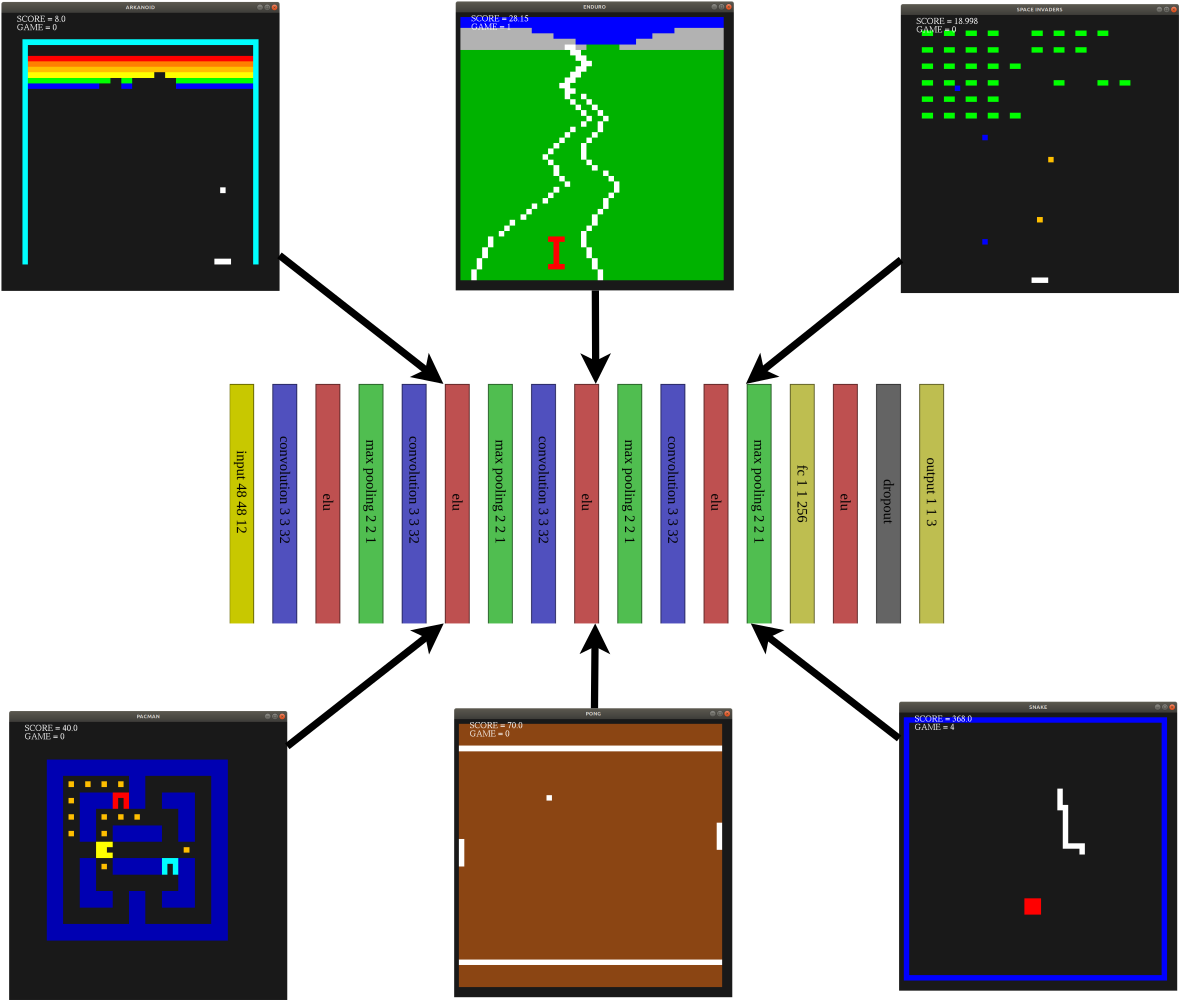
\includegraphics[width=0.5\textwidth]{diagrams/multi_dqn.png}
\caption{Multi DQN can play six games with the same weights}

\end{figure}

\section{Experiment setup}

{\bf Network input}:
Last 4 frames, width = 48, height = 48.


{\bf Network architecture}:
Following state of the art (cite VGG Net, ResNet), we used only 3x3 kernels, instead of (cite Atari DQN, Doom, with 8x8 kernels). As activation
function the ELU is choosen, with $\alpha = 0.1$.
After four convolution and pooling layers, the full connected layer with 256 neurons is used.
On the last layer the linear activation is used. We also tried network without 256 FC layer - to reduce amount of parameters, but the training was much slower.

Proposed network architecture is : \\
$IN48\times 48\times 12 - C3\times 3\times 32 - P2\times 2 - C3\times 3\times 32 - P2\times 2 - C3\times 3\times 32 - P2\times 2 - C3\times 3\times 32 - P2\times 2 - FC256 - FC_{actions}$

Hyperparmaters of network were choosen as :
\begin{itemize}
    \item learning rate $\eta = 0.001$
    \item L1 and L2 regularization $\lambda _1 = \lambda _2 = 0.0000001$
    \item dropout $0.02$ (only after FC256 layer)
    \item minibatch size 32 for single DQN, 128 for multi DQN
\end{itemize}

\newpage
\section{Results}



\begin{figure}[htb!]
    \centering
    \subfloat[Arkanoid]{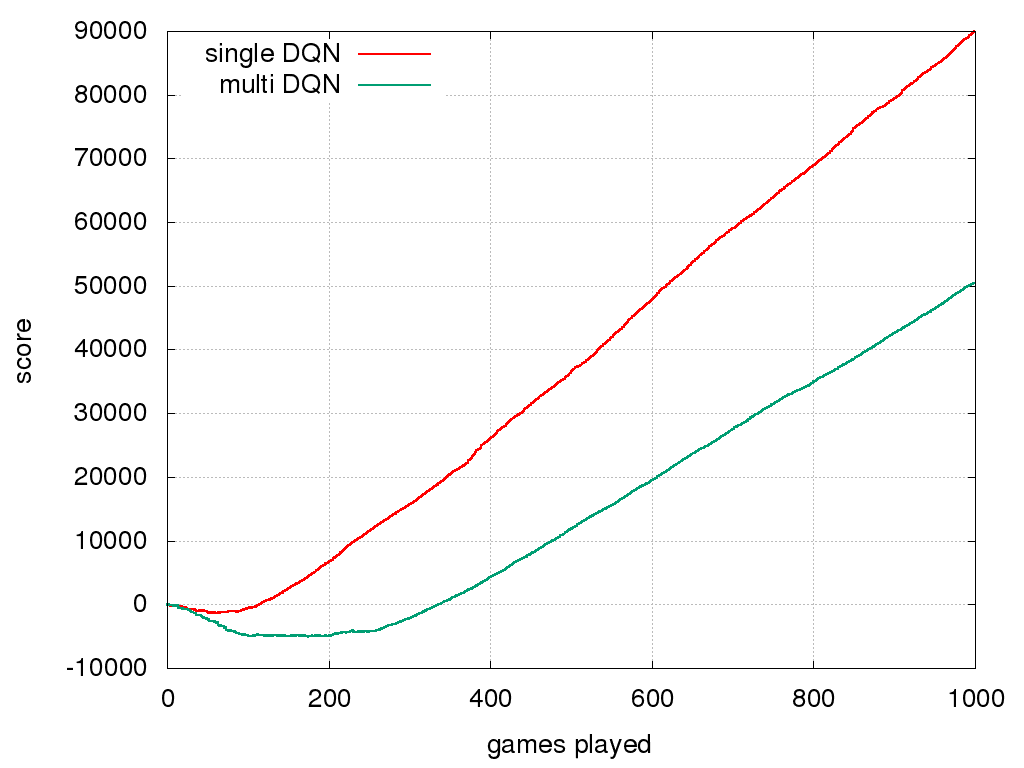
\includegraphics[width=5cm]{results/progress_training_arkanoid.png}}\hfil
    \subfloat[Enduro]{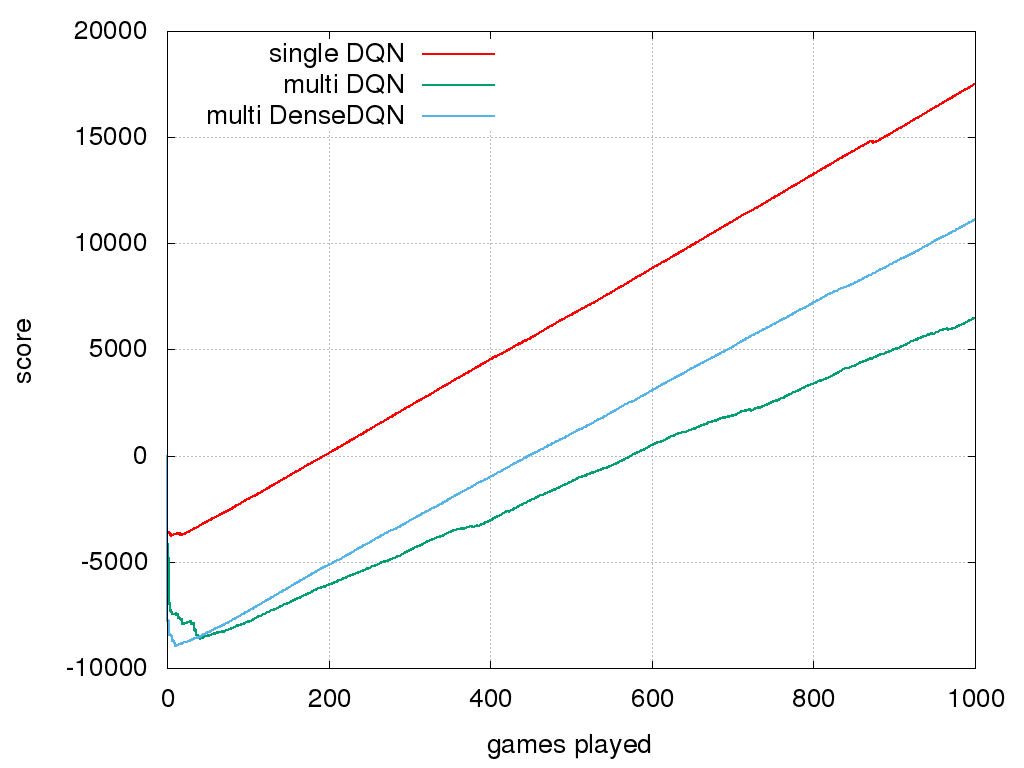
\includegraphics[width=5cm]{results/progress_training_enduro.png}}\hfil
    \subfloat[Invaders]{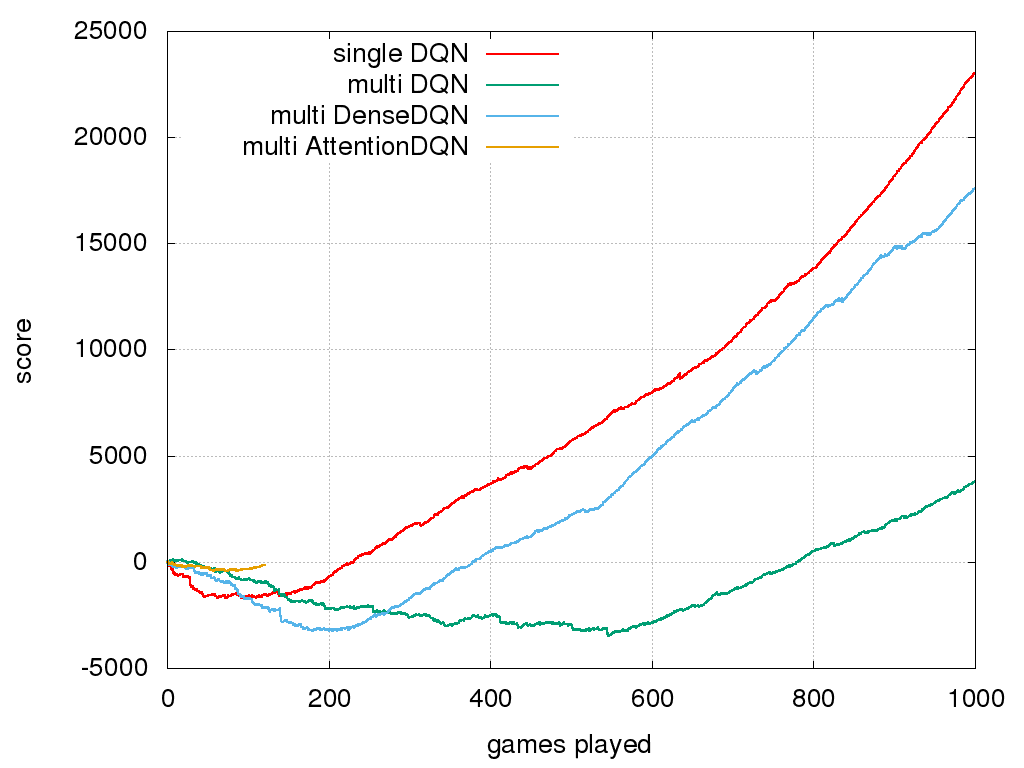
\includegraphics[width=5cm]{results/progress_training_invaders.png}}

    \subfloat[Pacman]{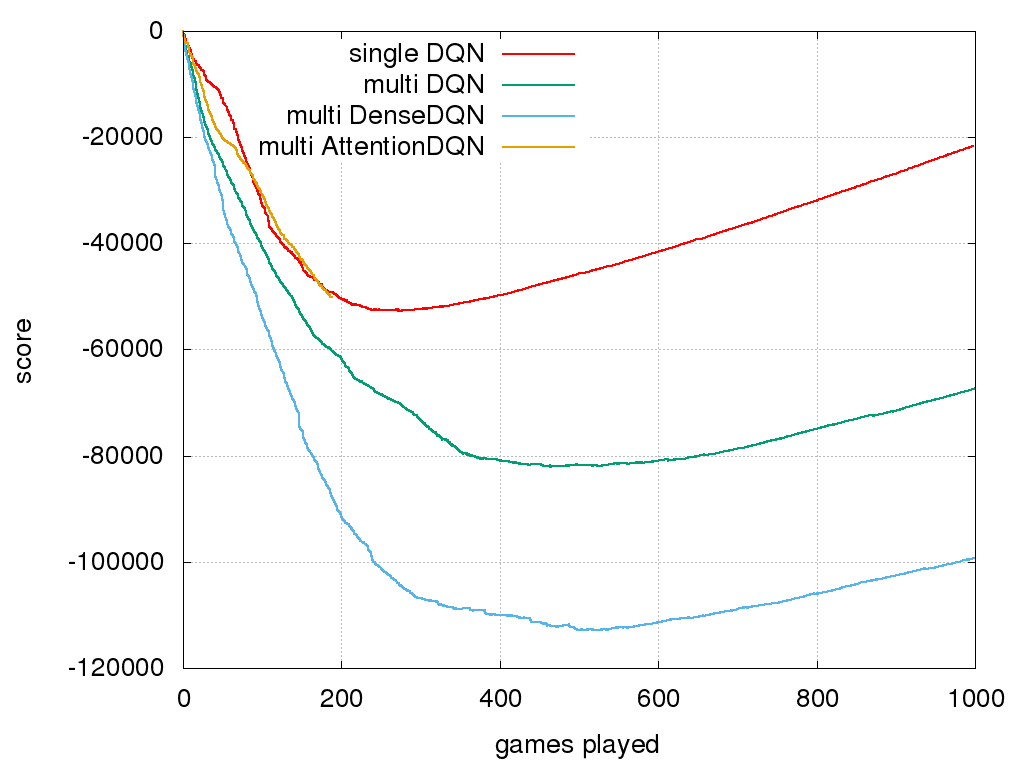
\includegraphics[width=5cm]{results/progress_training_pacman.png}}\hfil
    \subfloat[Pong]{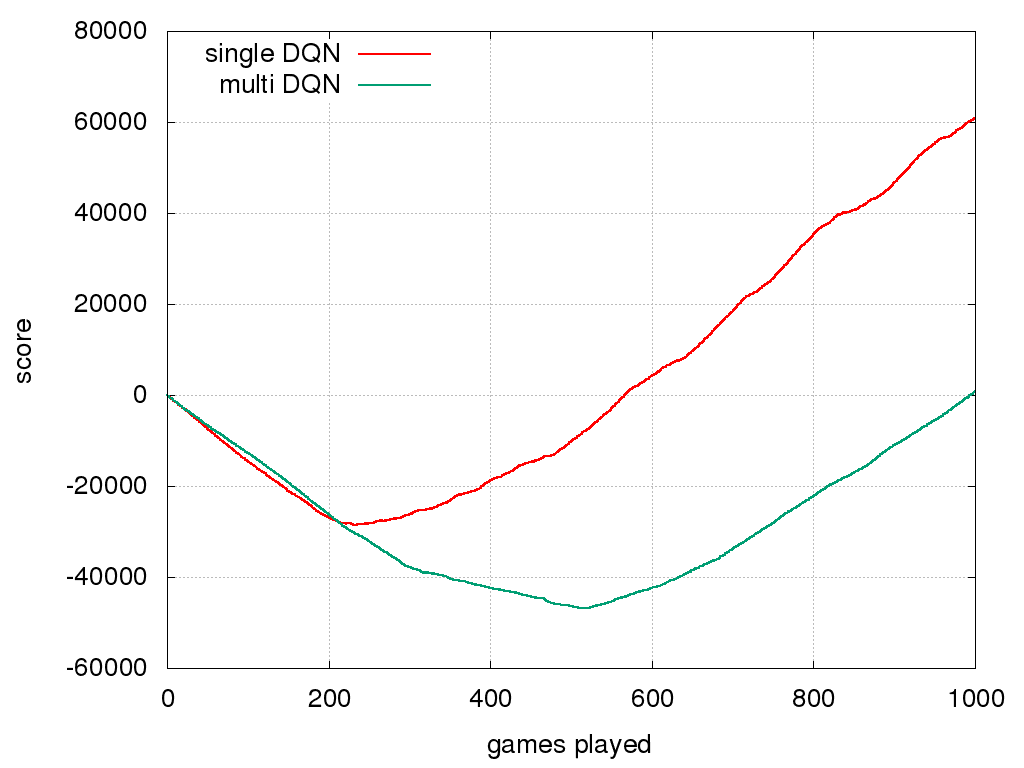
\includegraphics[width=5cm]{results/progress_training_pong.png}}\hfil
    \subfloat[Snake]{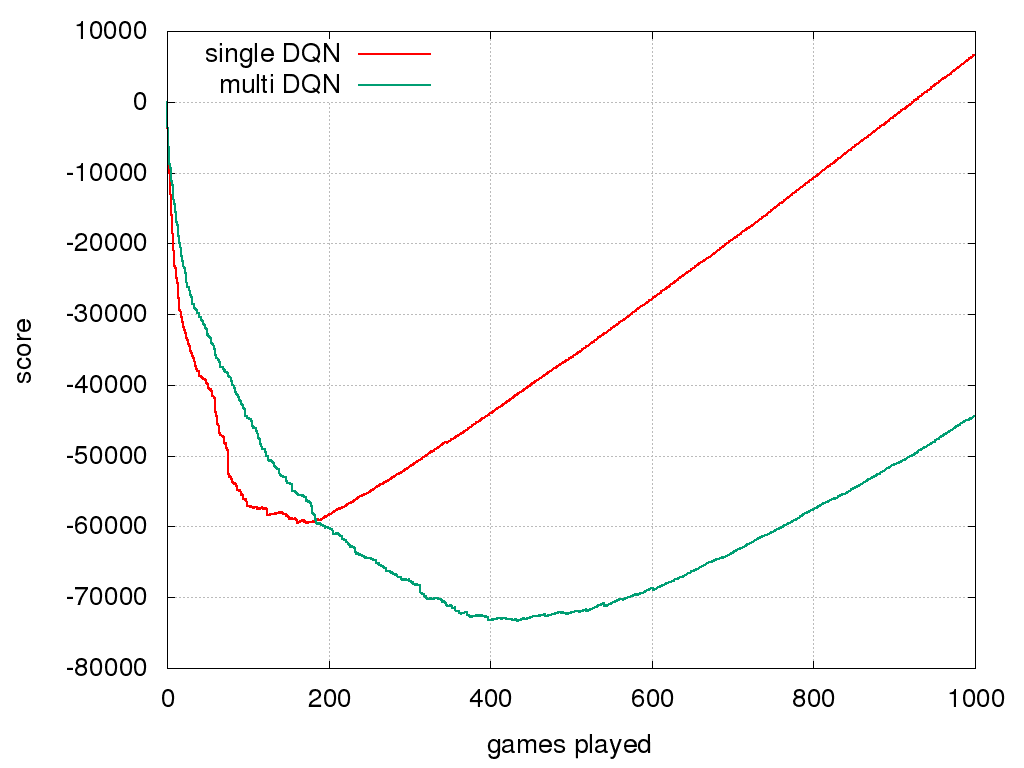
\includegraphics[width=5cm]{results/progress_training_snake.png}}
    \caption{Training score result for first 1000 games}\label{img:score_result}
\end{figure}


\begin{figure}[htb!]
    \centering
    \subfloat[Single DQN max activity]{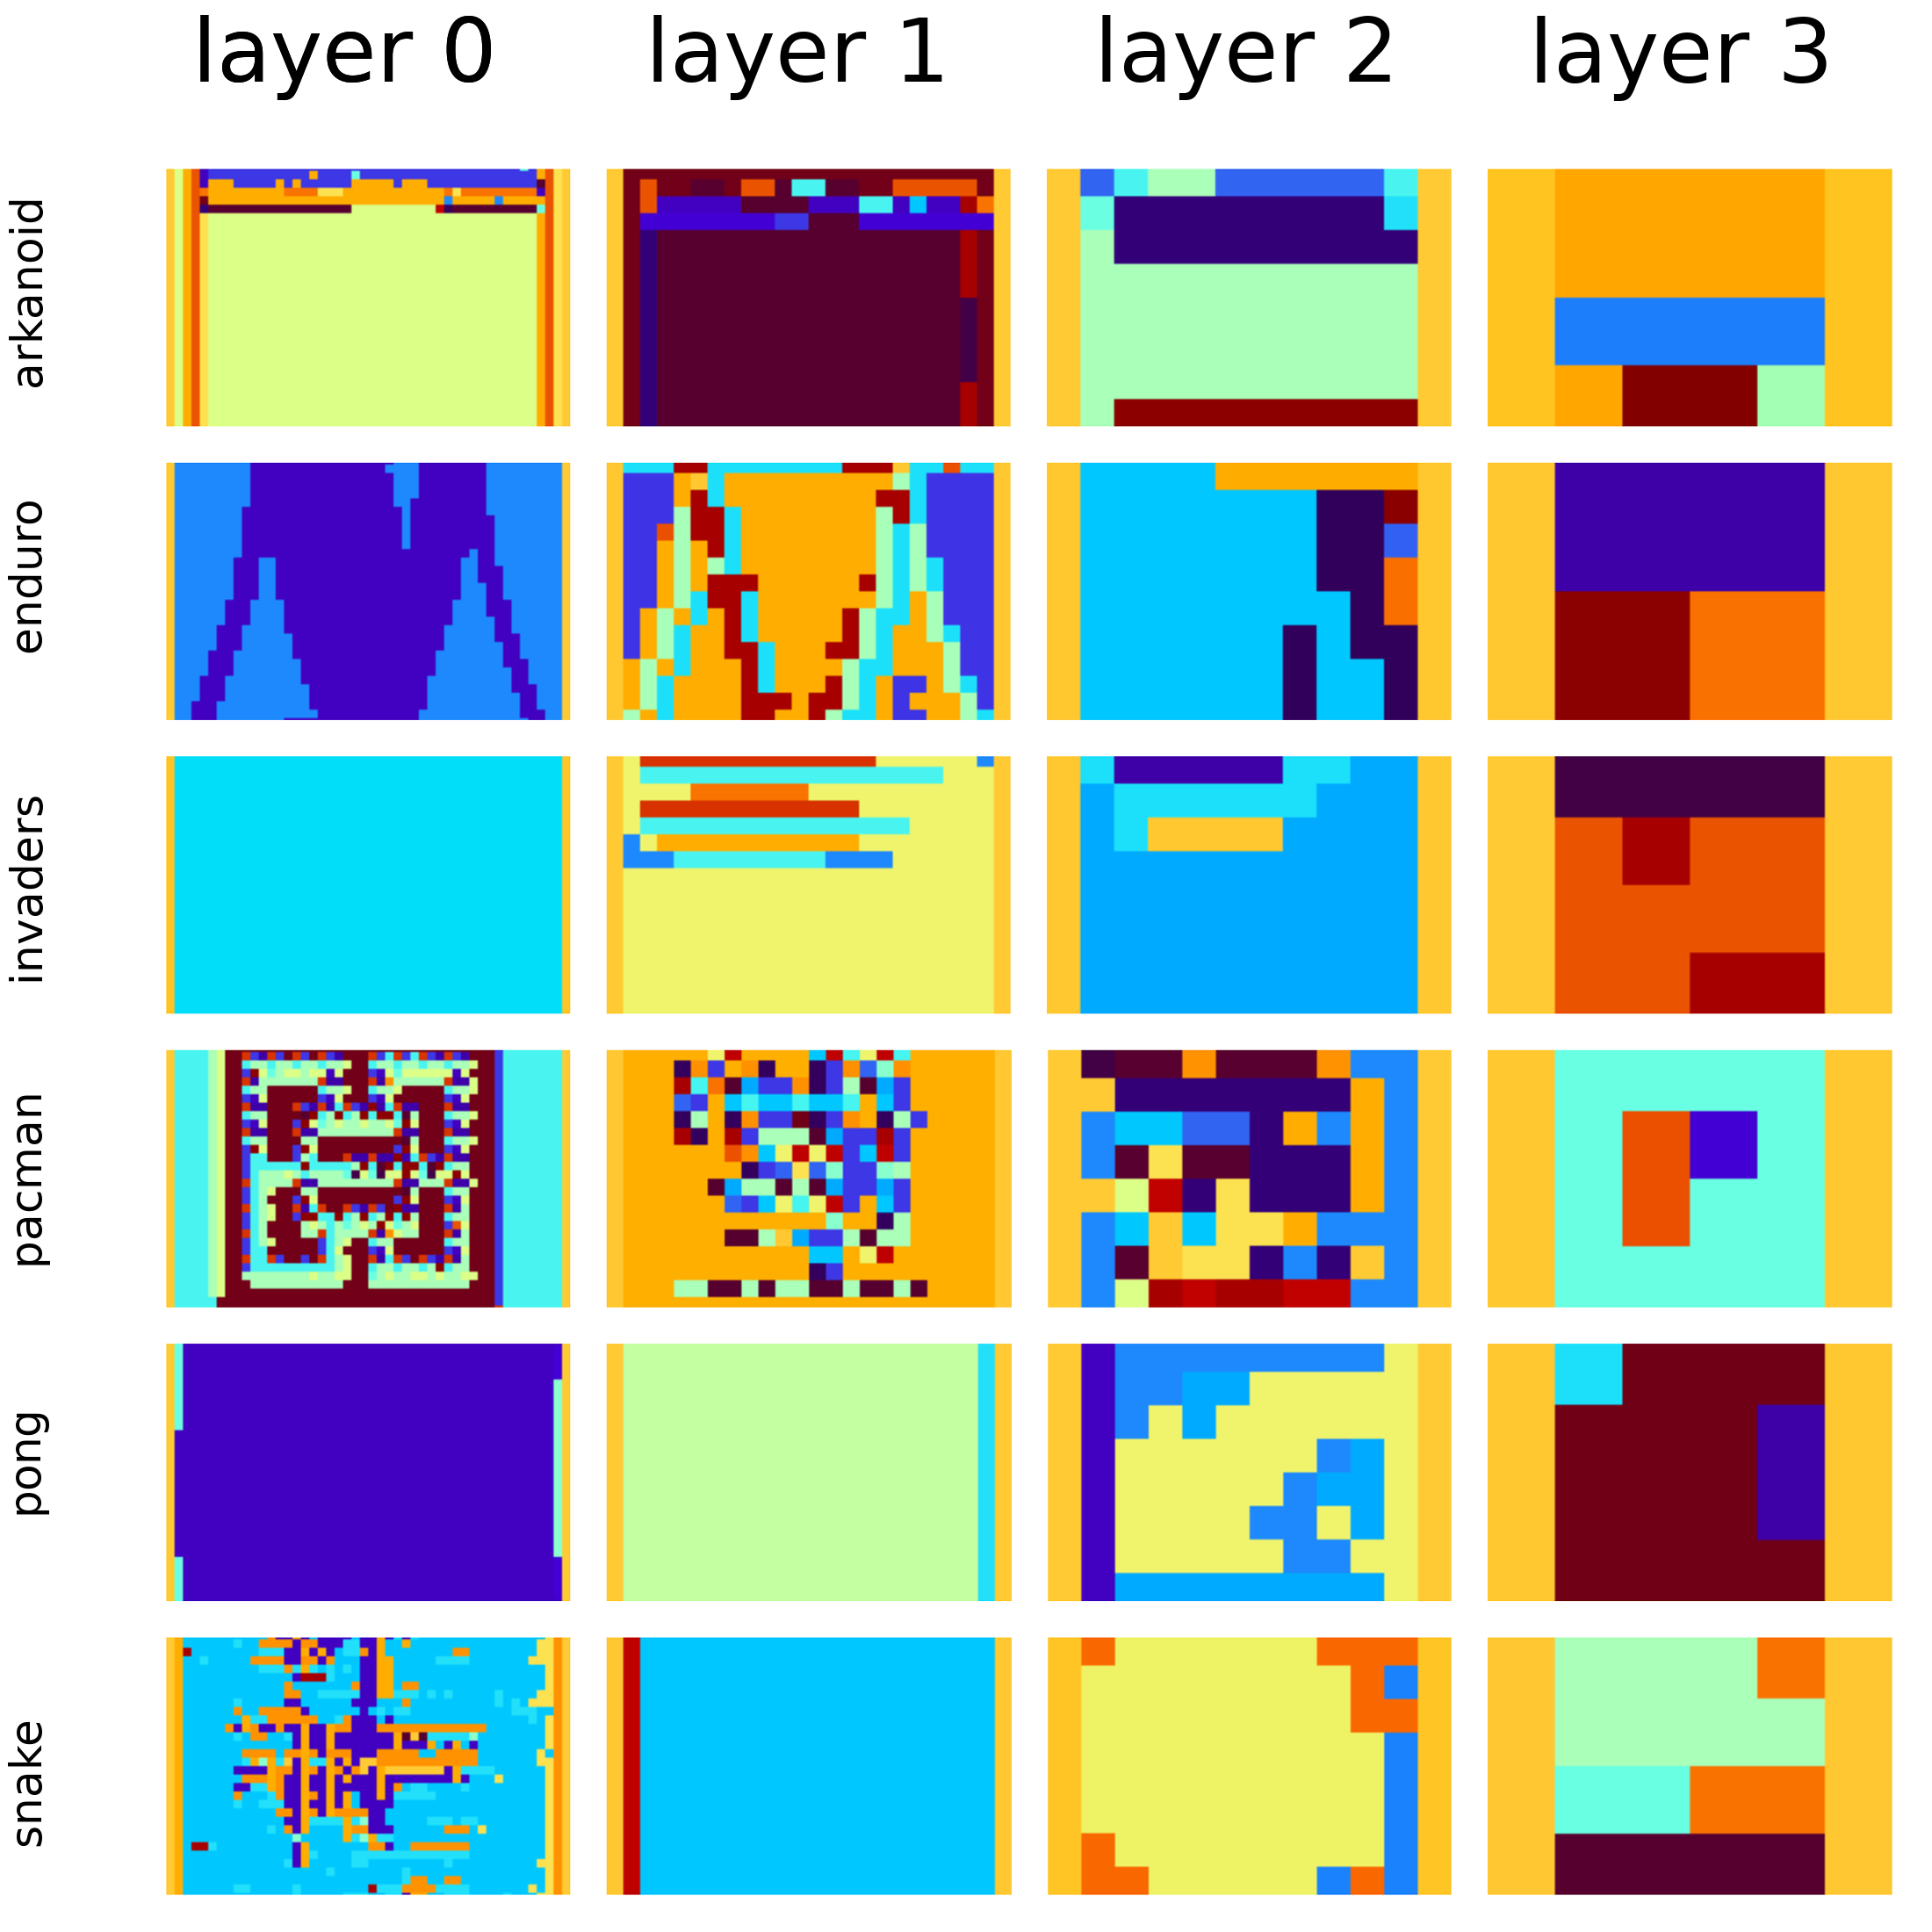
\includegraphics[width=6cm]{results/activity/single_net_max_desc.png}}\hfil
    \subfloat[Multi DQN max activity]{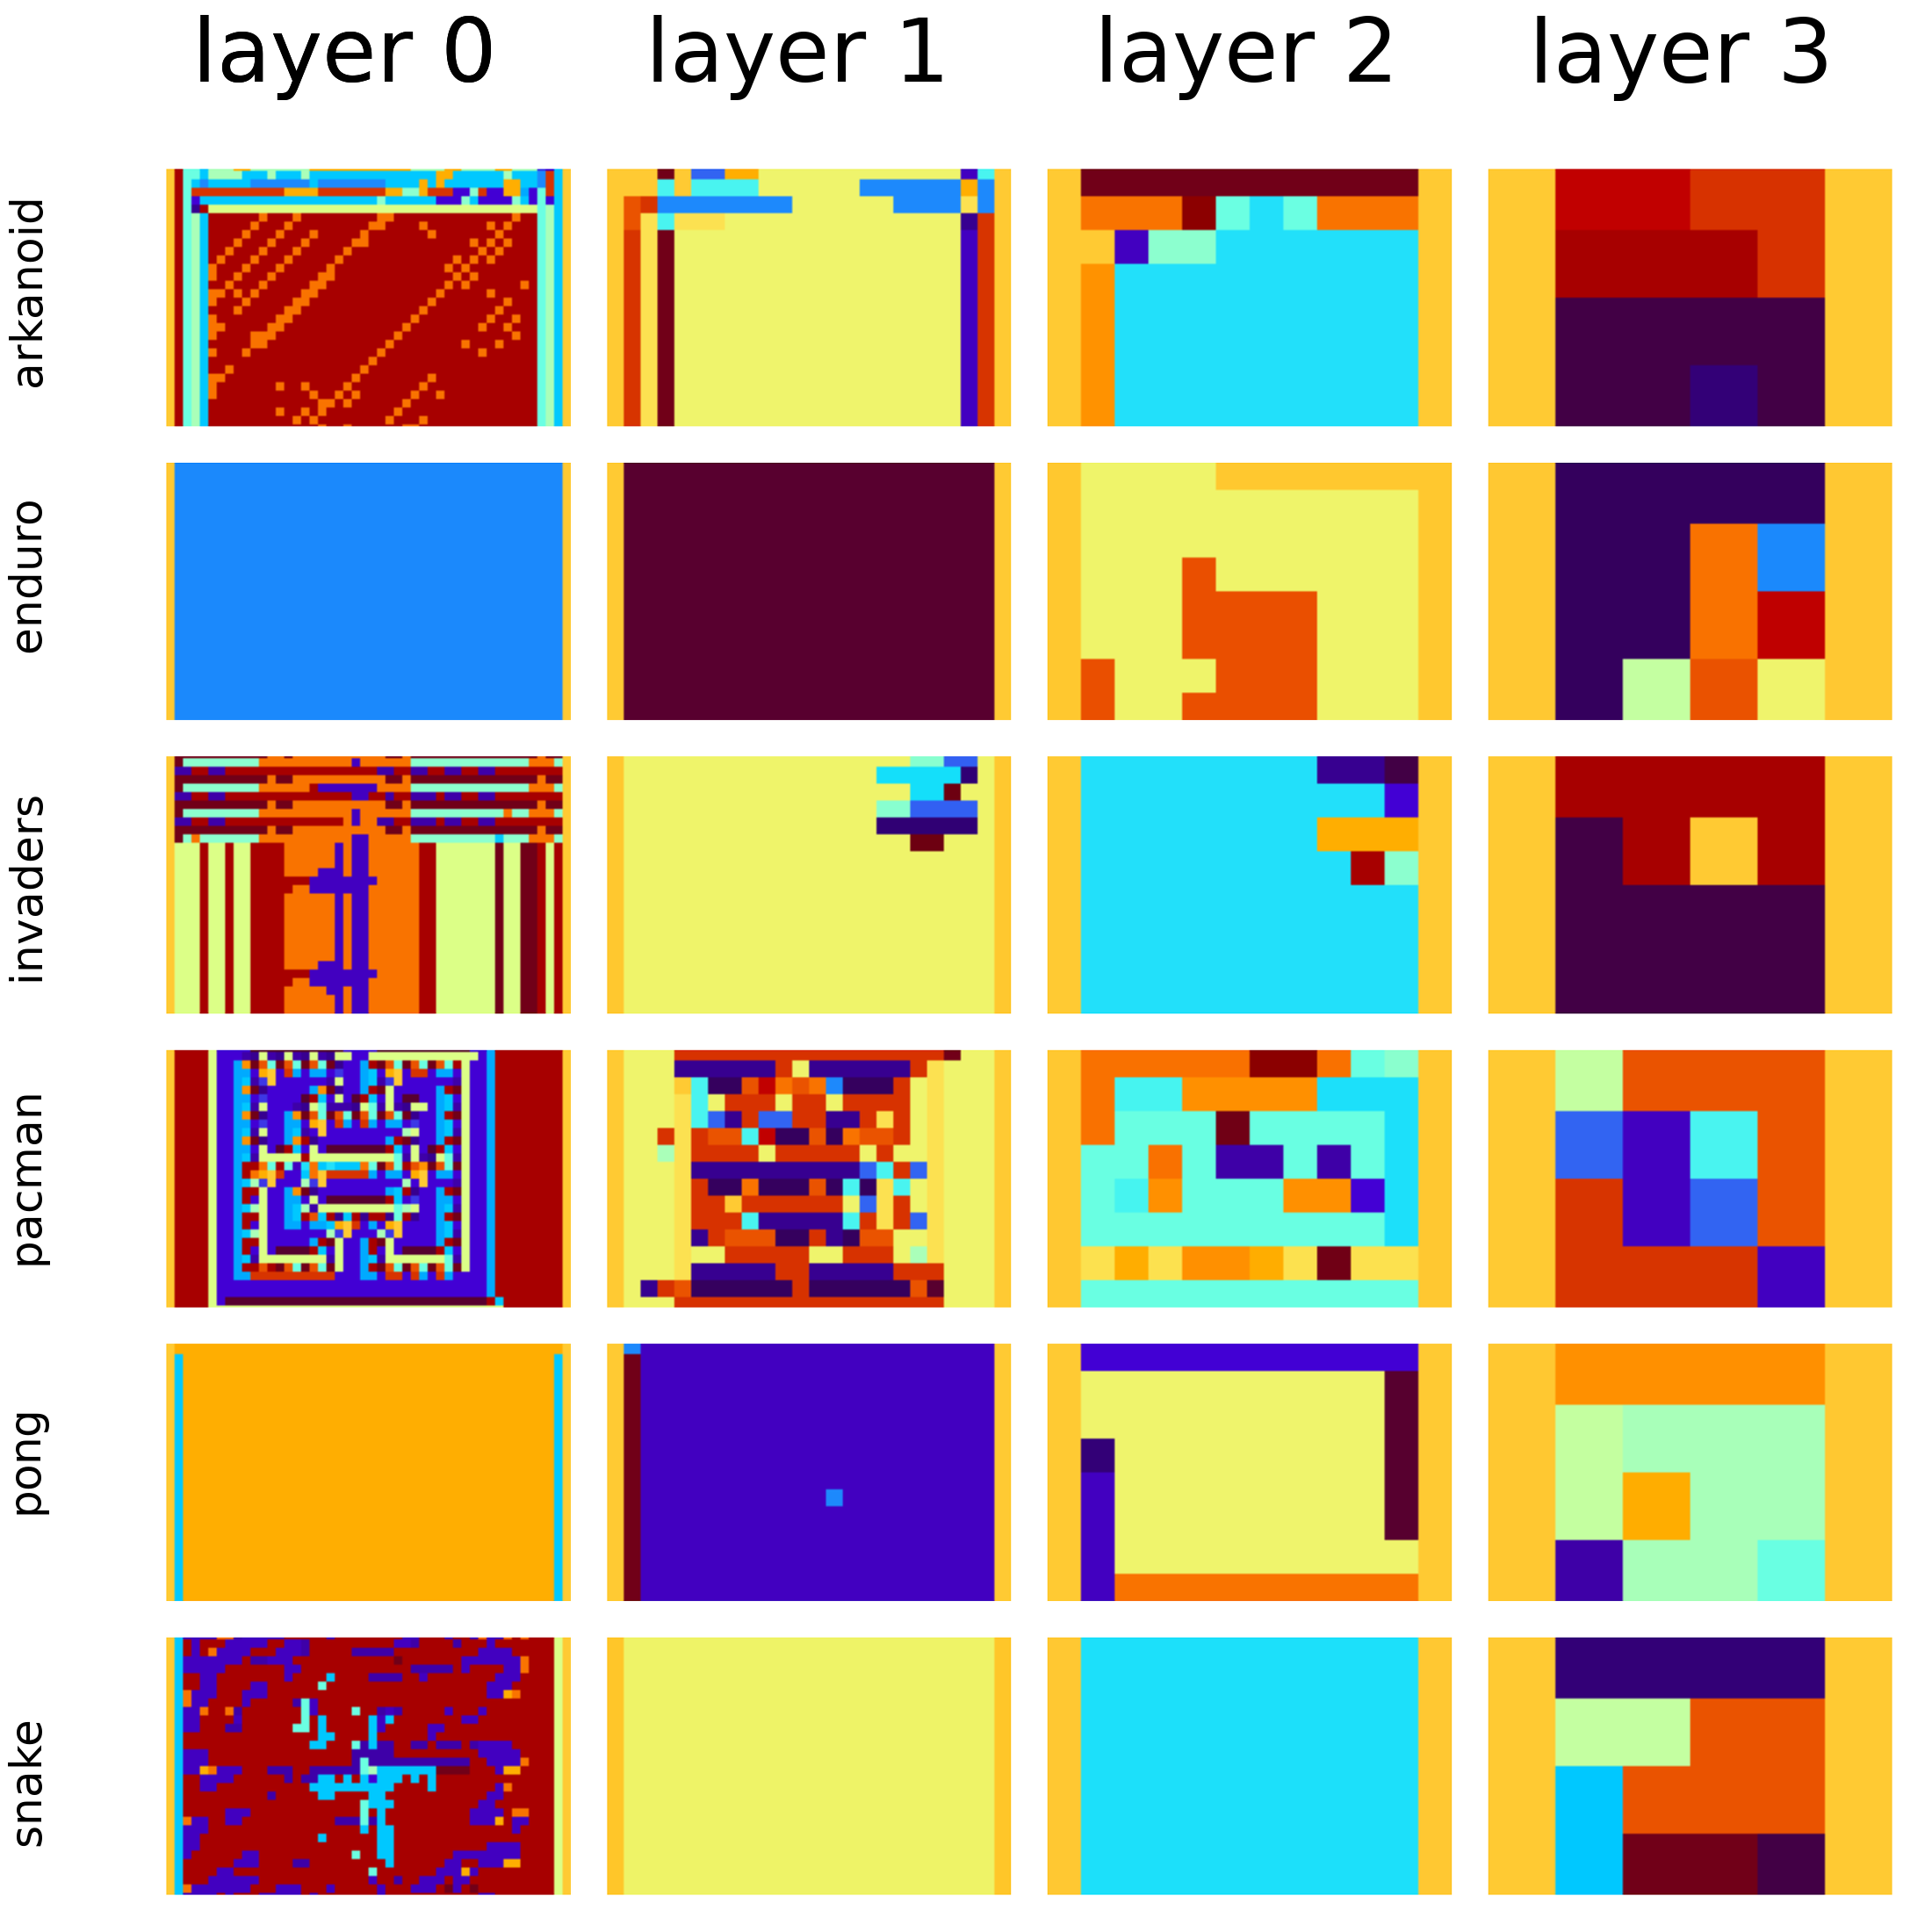
\includegraphics[width=6cm]{results/activity/multi_net0_max_desc.png}}\hfil

    \subfloat[Single DQN average activity]{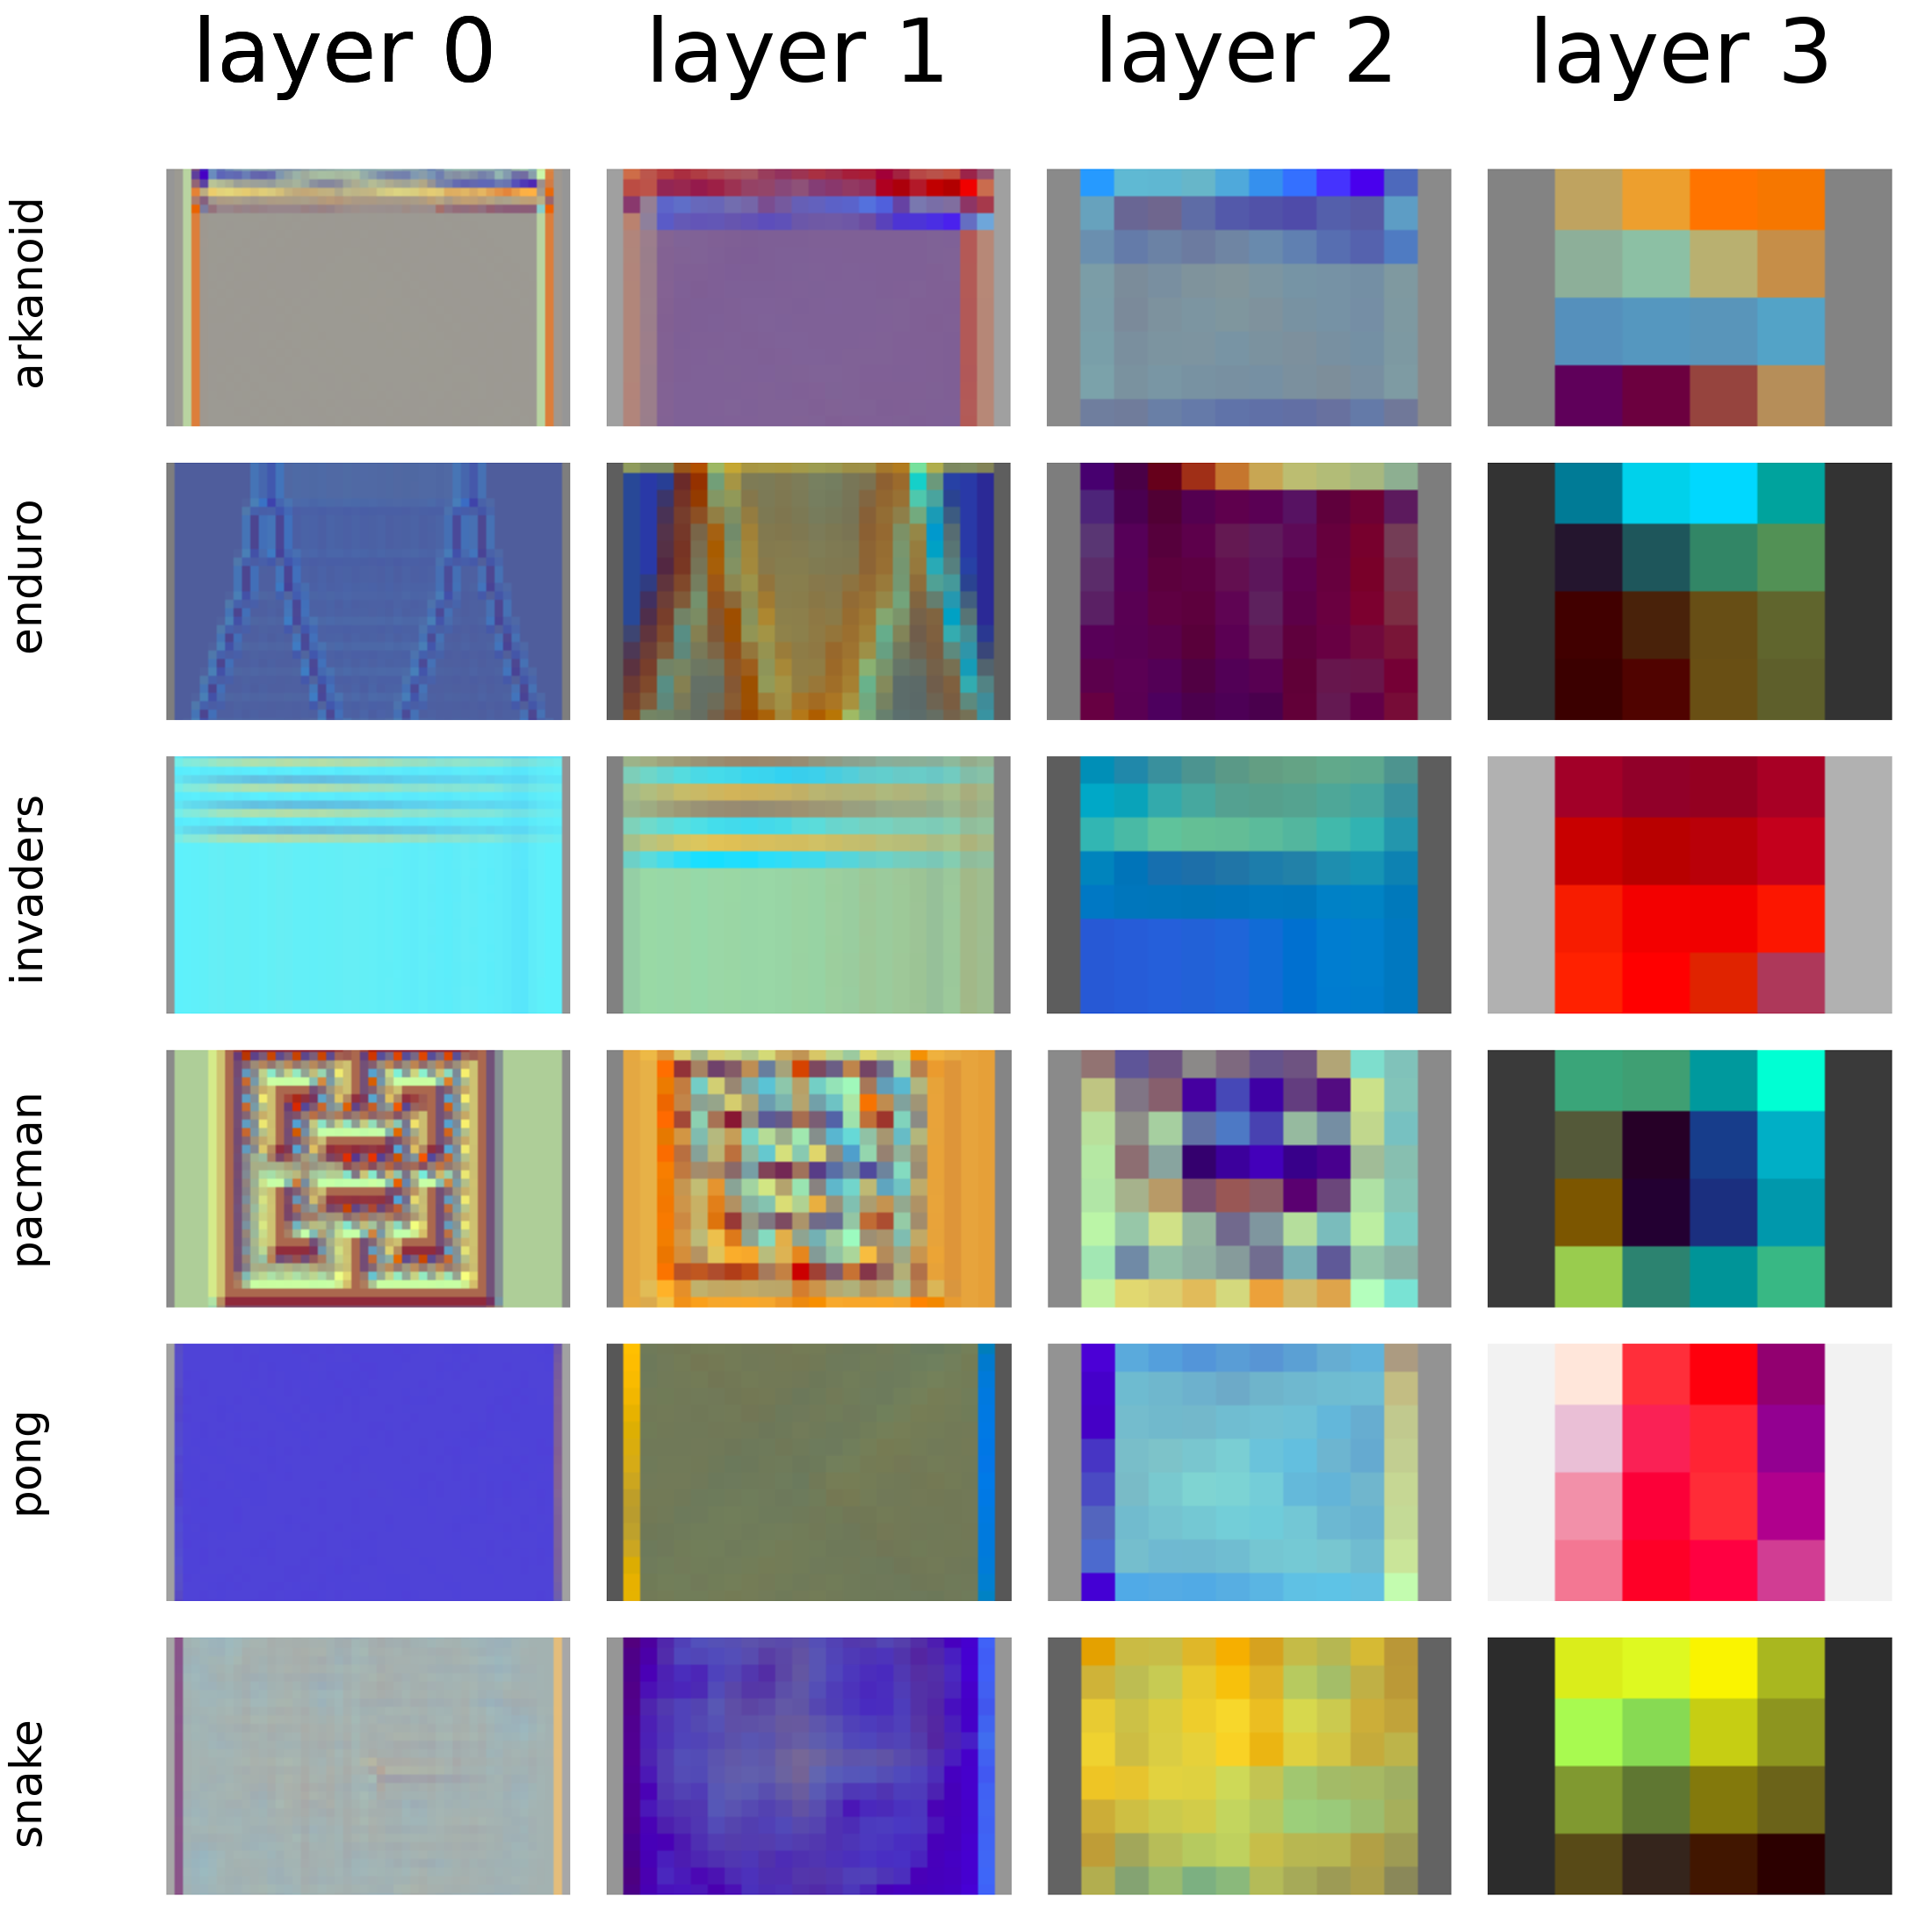
\includegraphics[width=6cm]{results/activity/single_net_average_desc.png}}\hfil
    \subfloat[Multi DQN average activity]{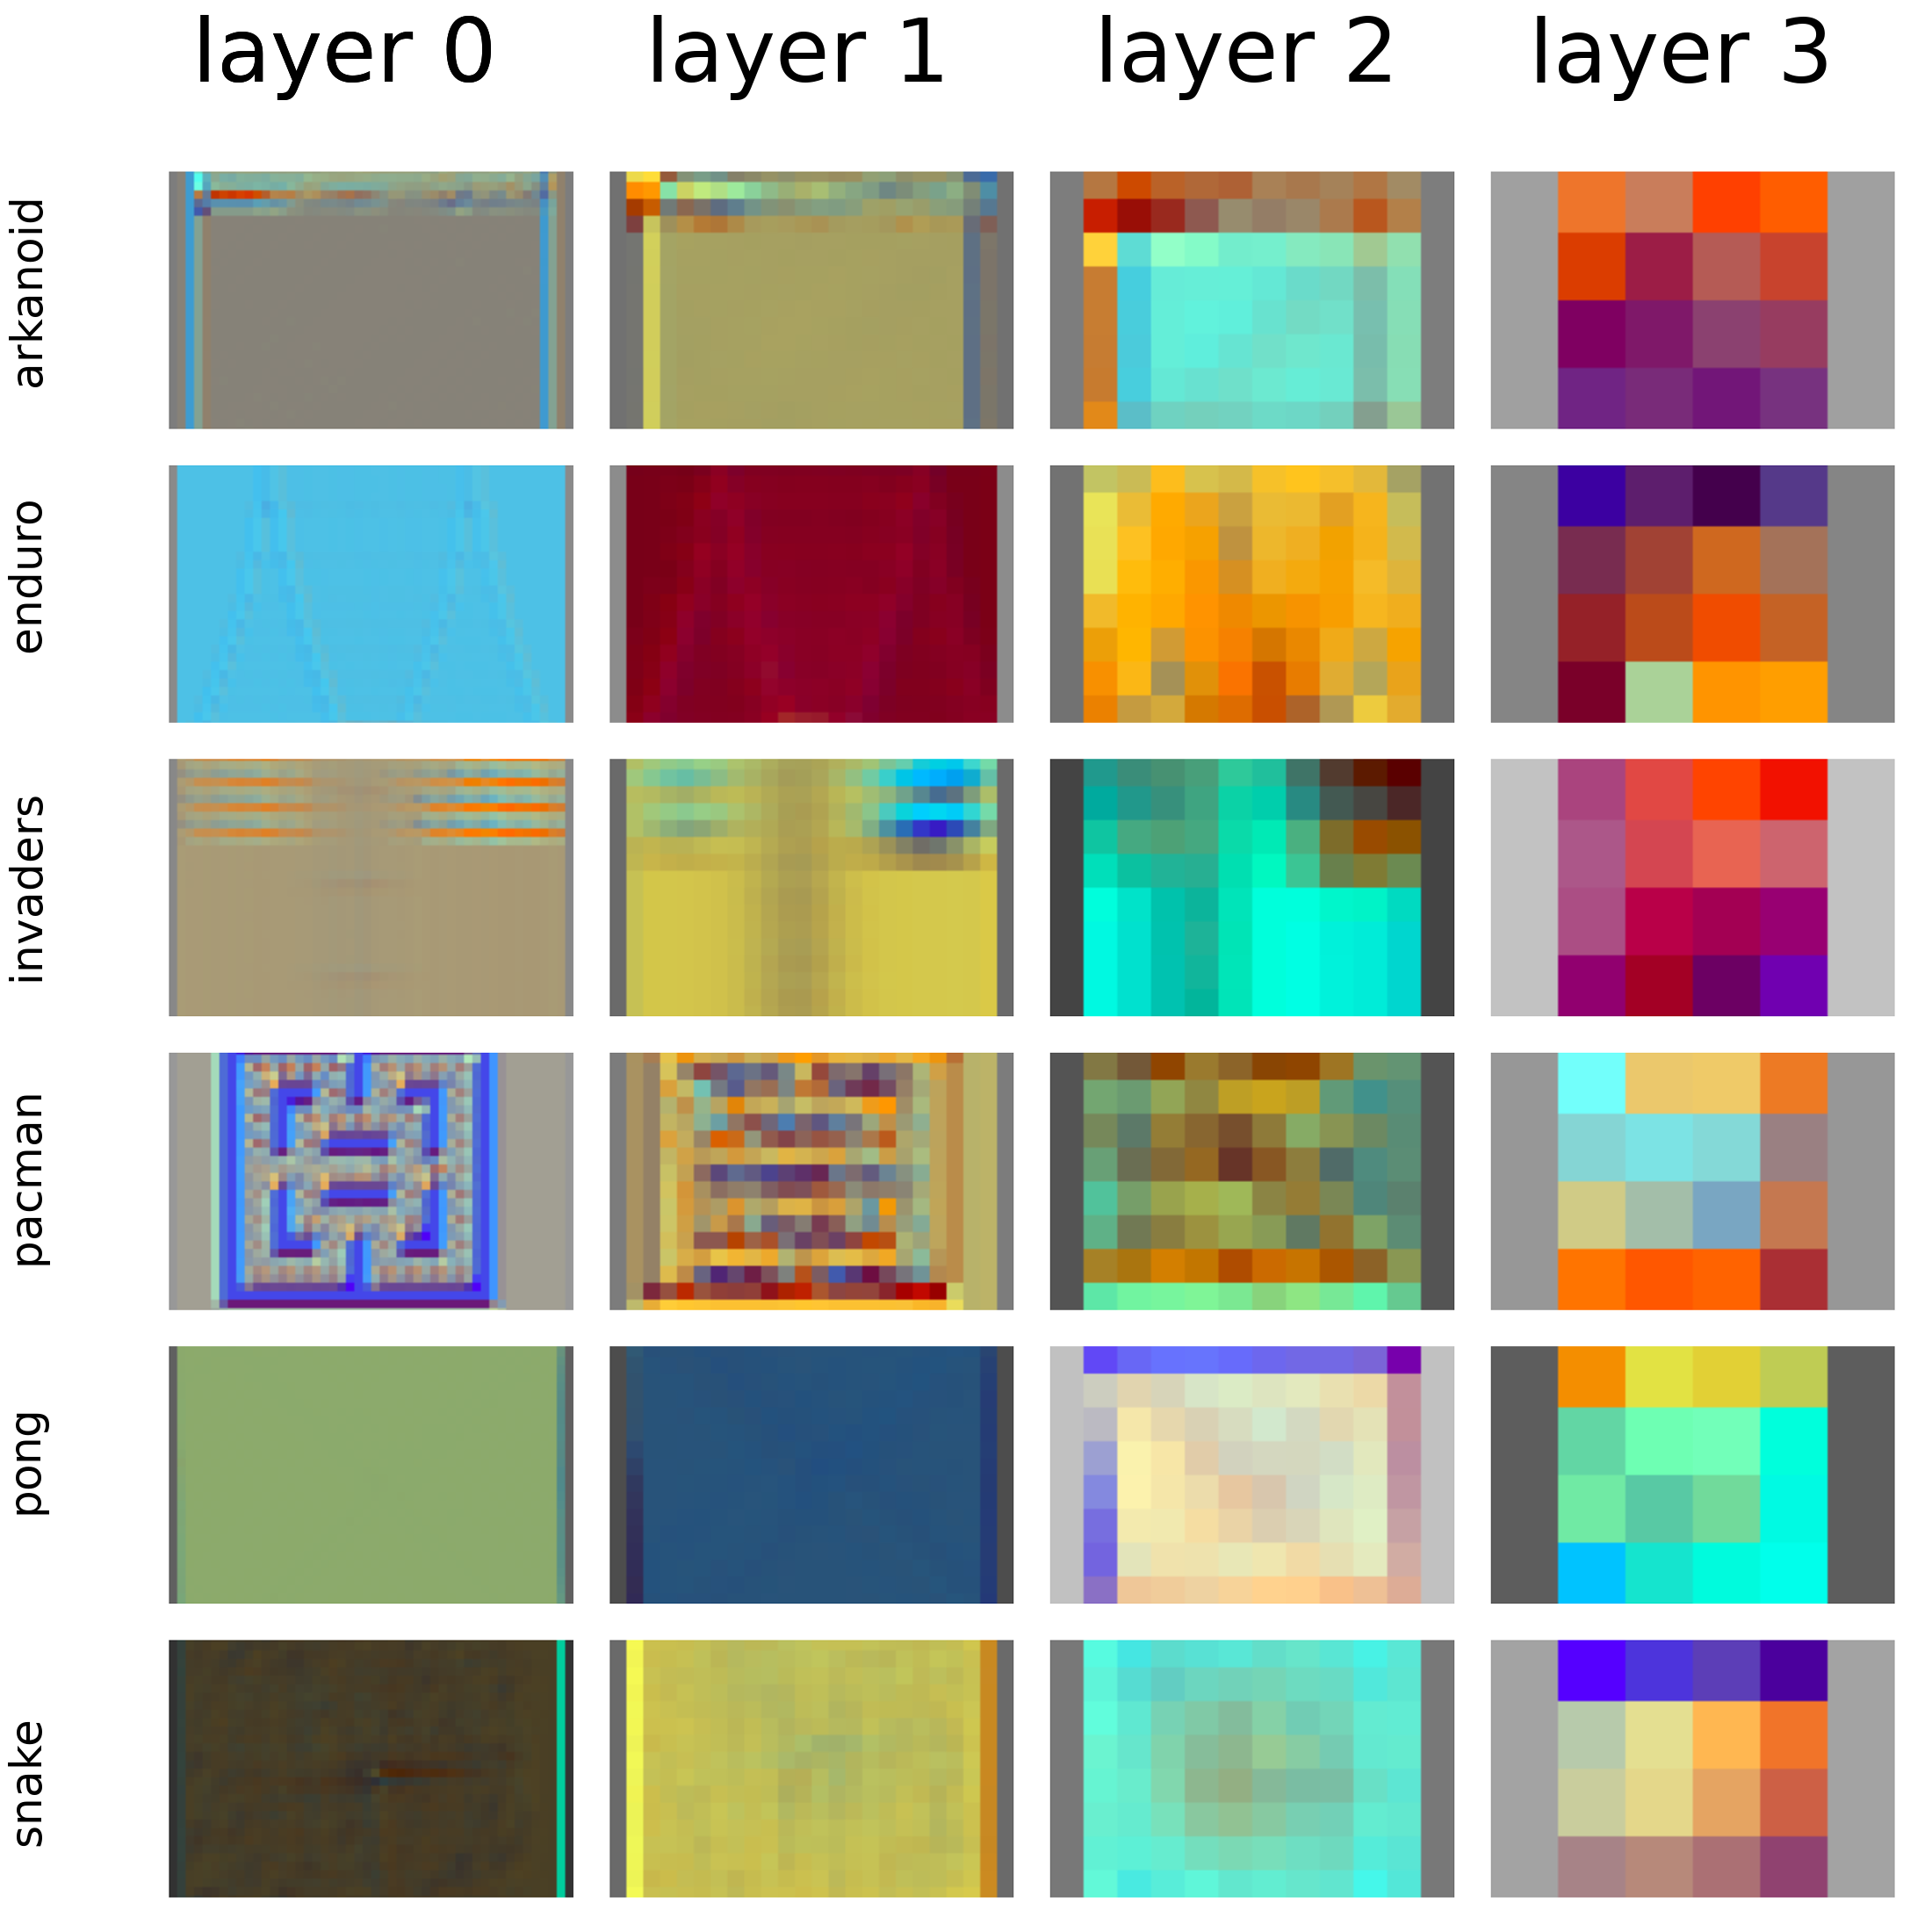
\includegraphics[width=6cm]{results/activity/multi_net0_average_desc.png}}\hfil

    \caption{Feature maps activity}\label{img:activity}
\end{figure}




\end{document}
